\documentclass[conference]{IEEEtran}
\IEEEoverridecommandlockouts
\usepackage{amsmath,amssymb}
\usepackage{graphicx}
\usepackage{booktabs}
\usepackage[hidelinks]{hyperref}
\usepackage{url}

\begin{document}

\title{PhishGuard: An Explainable Hybrid System for Phishing Email Triage}

\author{\IEEEauthorblockN{Akshay Kumar Bolusani}
\IEEEauthorblockA{ProjectKaro, Hyderabad, India\\
akshaykumarbolusani@gmail.com\\
\url{https://github.com/AkshayKumarBolusani/PhishGuard-AI-Explainable-Hybrid-Phishing-Detection-System}}
}

\maketitle

\begin{abstract}
Security operations centers drown in suspicious email. Every false positive
costs an analyst minutes they do not have. And a bare verdict such as
``phishing: 92\%'' is useless in an incident report. There is nothing to
quote and nothing to defend. PhishGuard is an open-source triage platform
built around that reality. Its detection core pairs a deterministic 29-rule
heuristic engine with TF-IDF statistical classifiers in a fixed weighted
ensemble, and every decision ships with an analyst-readable report
explaining it.

We benchmarked the core on five public corpora, 108,116 emails in total:
TREC 2007, CEAS 2008, Nazario, Nigerian fraud, and SpamAssassin. Stratified
5-fold cross-validation, identical splits for every model, no exceptions.
Three baselines: a PILFER-style heuristic feature set with random forest,
TF-IDF with logistic regression, and TF-IDF with a linear SVM.

The hybrid reaches F1 scores of 0.908--0.986 and takes the best precision on
four of five corpora (0.985--1.000). The TF-IDF SVM wins F1 on all five
(0.984--0.998). That gap is the finding, not an embarrassment. The rule
layer trades 1 to 14 points of recall for precision and per-indicator
evidence. Where false alarms are expensive, that is a trade worth making.
Code, protocol, and results are public.
\end{abstract}

\begin{IEEEkeywords}
phishing detection, explainable AI, hybrid systems, SOC triage, email security
\end{IEEEkeywords}

\section{Introduction}
Phishing remains the most common first foothold in enterprise breaches. The
detection side of the problem is well studied. The triage side is not. Once
something looks suspicious, an analyst gets minutes to decide: escalate,
contain, or dismiss. Two things decide whether a tool survives that moment.
Precision comes first. A false positive is never free. It burns analyst time,
breeds alert fatigue, and slowly teaches the team to ignore the tooling.
Evidence comes second. A score with no reasoning cannot go into an incident
report. The analyst needs to see why, in words they can quote.

The literature attacked detection from both ends. Fette \textit{et al.}'s
PILFER combined ten hand-crafted deception features with machine learning
\cite{pilfer}. Zhang \textit{et al.}'s CANTINA derived TF-IDF lexical
signatures from page content and checked them against a search engine
\cite{cantina}. URL-lexical ML pipelines have held up as a durable baseline
ever since \cite{sahingoz2019}. Then explainability became a goal in its own
right. EXPLICATE couples a classifier with LIME/SHAP explanations rendered
into plain language by a large language model \cite{explicate}. What we could
not find was an open, deployable triage system aimed at the analyst instead
of the end user, evaluated on public corpora, that reports the full cost of
bolting a deterministic rule layer onto statistical classifiers rather than
claiming a win on accuracy.

PhishGuard is that system. A FastAPI/React/MongoDB platform whose detection
core fuses a 29-rule heuristic engine with TF-IDF classifiers under a fixed
weighted vote, with LLM-written analyst reports on every verdict. Three
contributions. First, the system itself, designed around precision and
evidence for SOC workflows. Second, a public benchmark of the detection core
on five standard corpora, 108,116 emails, against three baselines, all on
identical cross-validation splits. Third, an honest account of where the
hybrid helps (precision, explainability) and where it hurts (recall, F1)
next to pure statistical models. Everything needed to reproduce the work is
released.

Section~II covers related work, Section~III the architecture, Section~IV the
evaluation protocol, Section~V the results, Section~VI limitations and future
work, and Section~VII concludes.

\section{Related Work}
\textbf{Heuristics and statistical detection.} PILFER \cite{pilfer}
introduced ten features aimed at deceptive technique: IP-based URLs, domain
age, mismatched link targets, link and domain counts. With SVM and
random-forest classifiers it reported over 96\% phishing detection at roughly
0.1\% false positives against the filters of its day. CANTINA \cite{cantina}
took the content route instead, deriving TF-IDF lexical signatures from page
text and verifying them through a search engine. Sahingoz \textit{et al.}
\cite{sahingoz2019} later showed that URL-lexical features with classical
classifiers remain competitive. Our PILFER-style baseline reimplements that
heuristic spirit with ten URL/HTML features. Domain-age and WHOIS lookups are
left out; the evaluation ran with no network access.

\textbf{Explainable phishing detection.} EXPLICATE \cite{explicate} pairs a
classifier built on domain-specific features with a dual LIME/SHAP
explanation layer, translated by DeepSeek v3 into accessible language. It
reports 98.4\% accuracy alongside measured explanation quality, shipped as a
GUI and browser extension for end users. The audience is the difference.
PhishGuard writes for the SOC analyst: indicators with quoted matched text,
URL and sender findings, a recommended action. The explanation lives inside
an alert-triage workflow, not a consumer tool.

\textbf{Evaluation practice.} Too many detectors are evaluated on private or
single corpora. Comparison becomes impossible. The TREC Spam Track was an
early attempt at a shared framework with public corpora such as trec07p
\cite{trec07}. We evaluate on the public \textit{Phishing Email Curated
Datasets} collection (Zenodo DOI 10.5281/zenodo.8339691) \cite{phishcurated},
spanning the TREC 2007 and CEAS 2008 tracks plus Nazario, Nigerian-fraud, and
SpamAssassin messages. The exact protocol and code are published with this
paper.

\section{System Architecture}
\begin{figure}[htbp]
\centering
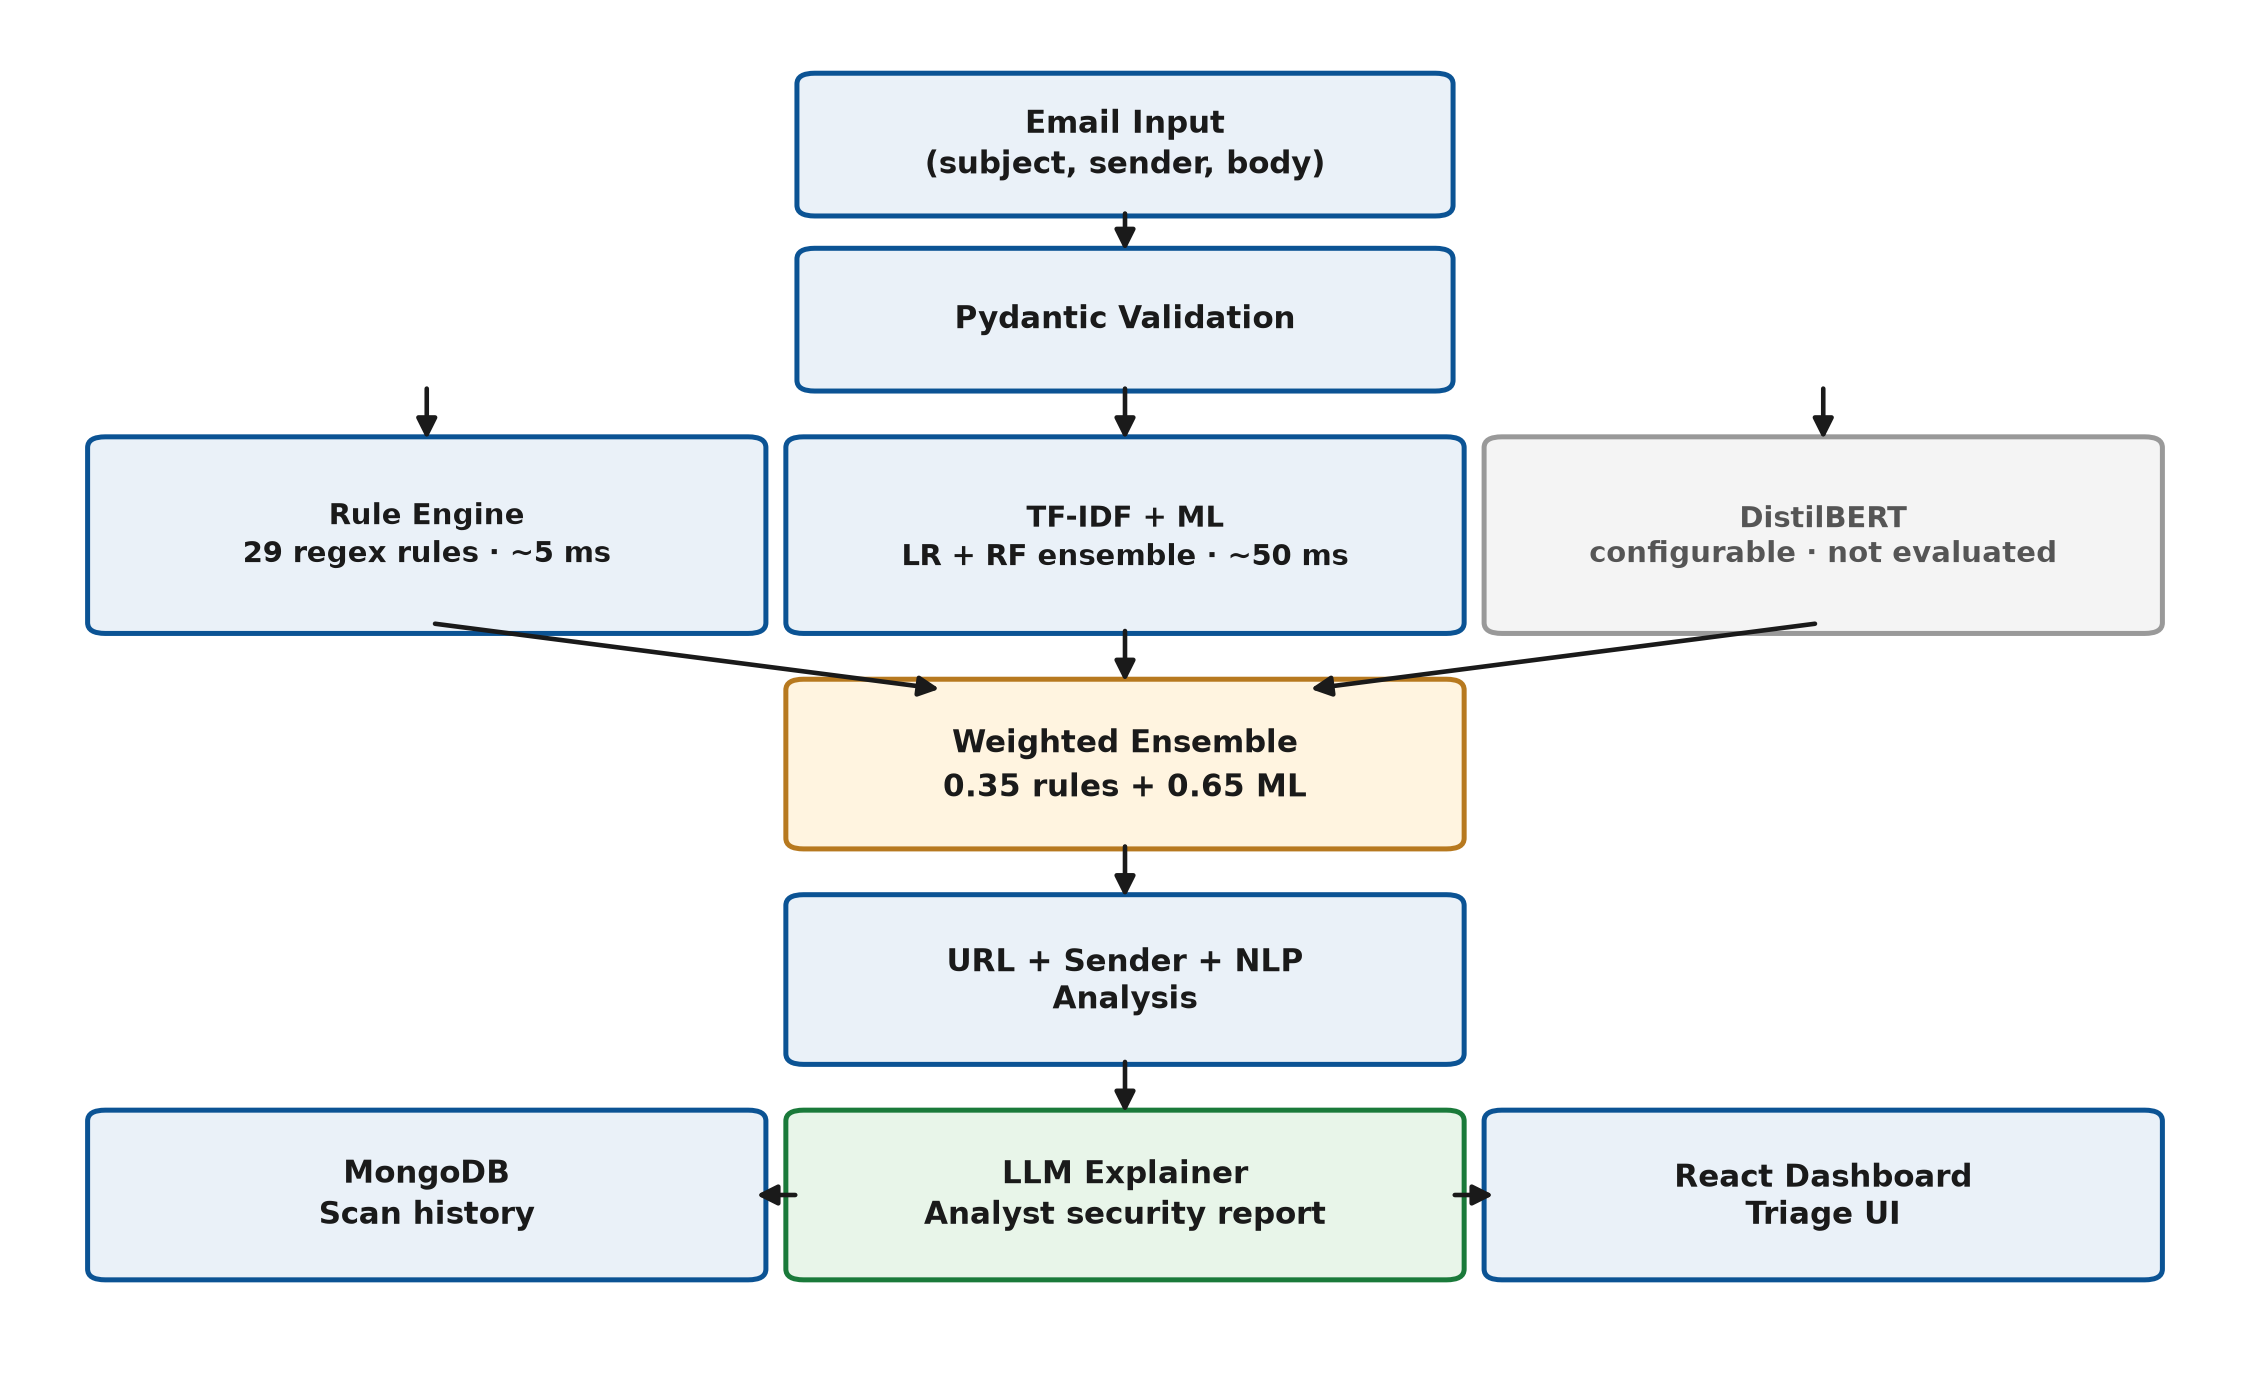
\includegraphics[width=\columnwidth]{fig_architecture.png}
\caption{PhishGuard pipeline. Email input passes validation, three detection
layers (29-rule engine, TF-IDF ML ensemble, configurable DistilBERT), a fixed
weighted ensemble, URL/sender/NLP analysis, and LLM explanation, served via
REST API with a React triage dashboard and MongoDB history.}
\label{fig:pipeline}
\end{figure}
Fig.~\ref{fig:pipeline} shows the pipeline. Three design goals shaped it. No
black boxes: whatever the system claims, the analyst must see why.
Deterministic signals fire fast and never depend on model state. And the
whole thing runs self-hosted, triaging each email in under a second.

\subsection{Rule Engine}
29 compiled regular-expression rules in ten categories (Table~\ref{tab:rules}).
Each match carries a severity, low to critical, and a confidence. A 0--100
risk score and 3-class probabilities (safe/suspicious/phishing) come from
severity-weighted aggregation. Typical latency is about 5\,ms per email.

\begin{table}[htbp]
\caption{Rule-engine categories (29 rules total).}
\label{tab:rules}
\centering
\footnotesize
\begin{tabular}{@{}lcl@{}}
\toprule
Category & Rules & Example pattern \\
\midrule
Urgency & 2 & ``act now'', ``within 24 hours'' \\
Threat & 3 & account suspension, legal threats \\
Credential harvesting & 3 & ``verify your password'' \\
Financial fraud & 5 & wire transfer, gift cards, crypto \\
Scam & 4 & lottery, tax refund, employment \\
Business-email compromise & 2 & CEO fraud, authority impersonation \\
Social engineering & 3 & emotional manipulation, curiosity bait \\
Link manipulation & 2 & ``click here'', attachments \\
Technical deception & 2 & brand impersonation, HTML obfuscation \\
Style & 3 & excessive caps, punctuation, grammar \\
\bottomrule
\end{tabular}
\end{table}

\subsection{ML Classifier}
TF-IDF over the email text, 10,000 features, 1--2 grams, sublinear TF. On top
of it sit logistic regression (C=1.0, class-weighted) and a random forest
(100 trees, max depth 12); their probabilities are averaged. Per-word
coefficients are exposed so the dashboard can show feature importance.
Typical latency is about 50\,ms.

\subsection{Ensemble}
Without the optional transformer, the final score is a fixed weighted vote:
\begin{equation}
P = 0.35 \cdot P_{\text{rules}} + 0.65 \cdot P_{\text{ML}},
\label{eq:ensemble}
\end{equation}
with $P_{\text{ML}}$ the averaged LR/RF probability. A DistilBERT layer
exists at weight 0.40, rebalancing the mix to 0.25/0.35/0.40, but it was not
trained for this build. It is switched off and excluded from every number
reported here. The weights are shipped defaults. They were not tuned on the
benchmark corpora.

\subsection{Explanation and Platform}
URL analysis scores every link for suspiciousness. Sender-trust scoring and
NLP urgency features complete the picture. An LLM explainer turns all of it
into an analyst-style report: executive summary, classification with
confidence, indicators with quoted evidence, URL and sender findings, attack
type, recommended actions. Around the core sits the platform. 17 REST
endpoints. A React dashboard with threat overview, split-pane scanner, and
searchable history exporting to CSV and JSON. MongoDB persistence. A feedback
endpoint where analysts can correct verdicts.

\section{Evaluation}
\subsection{Corpora}
Table~\ref{tab:corpora} summarizes the five corpora from \cite{phishcurated},
with 1 as phishing and 0 as legitimate. The TREC 2007 messages are the
track's public trec07p set, distributed under its standard evaluation
framework \cite{trec07}. Every file was MD5-checked against the
Zenodo-published checksums. Email text is subject plus body. HTML is kept
as-is so the link-manipulation features see the original markup.

\begin{table}[htbp]
\caption{Public evaluation corpora.}
\label{tab:corpora}
\centering
\footnotesize
\begin{tabular}{@{}lrrr@{}}
\toprule
Corpus & Messages & Phishing & Legitimate \\
\midrule
TREC\_07 (TREC 2007) & 53,757 & 29,399 & 24,358 \\
CEAS\_08 (CEAS 2008) & 39,154 & 21,842 & 17,312 \\
Nazario\_5 & 3,065 & 1,565 & 1,500 \\
Nigerian\_5 & 6,331 & 3,332 & 2,999 \\
SpamAssassin & 5,809 & 1,718 & 4,091 \\
\midrule
Total & 108,116 & 57,856 & 50,260 \\
\bottomrule
\end{tabular}
\end{table}

\subsection{Protocol}
Stratified 5-fold cross-validation, random state 42, with the \textbf{same
splits for every model}. The TF-IDF vectorizer is fit on each training fold
only. No test vocabulary leaks into training. We report accuracy, precision,
recall, and F1 on the phishing class, plus macro F1, all on pooled
out-of-fold predictions. The corpora are binary, so the system's
\textit{suspicious} class is not exercised here.

\subsection{Baselines}
\textit{PILFER-style:} ten hand-crafted URL/HTML features. IP-literal URL,
URL and domain counts, mismatched anchor/href, `@' in URL, subdomain depth,
HTML forms, JavaScript, longest URL, HTTPS ratio. Balanced random forest. It
reimplements the \cite{pilfer} idea, not the verbatim feature set.
\textit{TF-IDF+LR:} the system's own ML configuration, retrained per fold.
\textit{TF-IDF+SVM:} the same TF-IDF features with a balanced linear SVM.
\textit{PhishGuard hybrid:} the production rule engine, imported verbatim
from the codebase, combined per \eqref{eq:ensemble} and thresholded at 0.5.

The repository also ships a 130-email demonstration set, 50 safe, 35
suspicious, 45 phishing, for pipeline validation. Its cross-validation
figures (LR F1 $0.83 \pm 0.06$, RF F1 $0.85 \pm 0.09$) describe the demo.
They are \textbf{not} benchmark accuracy and are not presented as results.

\section{Results}
Table~\ref{tab:results} reports precision, recall, and F1 on the phishing
class per corpus. Fig.~\ref{fig:results} plots the F1 comparison.

\begin{table}[htbp]
\caption{Benchmark results: precision / recall / F1 on the phishing class
(pooled 5-fold out-of-fold predictions). Bold marks the best F1 and the best
precision within each corpus block.}
\label{tab:results}
\centering
\footnotesize
\begin{tabular}{@{}lccc@{}}
\toprule
Model & Precision & Recall & F1 \\
\midrule
\multicolumn{4}{@{}l}{\textit{TREC\_07 --- 53,757 emails}} \\
PILFER-style RF & 0.791 & 0.964 & 0.869 \\
TF-IDF + LR & 0.991 & 0.997 & 0.994 \\
TF-IDF + SVM & 0.995 & 0.998 & \textbf{0.996} \\
PhishGuard hybrid & \textbf{0.996} & 0.976 & 0.986 \\
\midrule
\multicolumn{4}{@{}l}{\textit{CEAS\_08 --- 39,154 emails}} \\
PILFER-style RF & 0.949 & 0.665 & 0.782 \\
TF-IDF + LR & 0.996 & 0.995 & 0.996 \\
TF-IDF + SVM & 0.998 & 0.998 & \textbf{0.998} \\
PhishGuard hybrid & \textbf{0.999} & 0.962 & 0.980 \\
\midrule
\multicolumn{4}{@{}l}{\textit{Nazario\_5 --- 3,065 emails}} \\
PILFER-style RF & 0.656 & 0.957 & 0.778 \\
TF-IDF + LR & 0.993 & 0.989 & 0.991 \\
TF-IDF + SVM & 0.997 & 0.994 & \textbf{0.996} \\
PhishGuard hybrid & \textbf{0.998} & 0.877 & 0.933 \\
\midrule
\multicolumn{4}{@{}l}{\textit{Nigerian\_5 --- 6,331 emails}} \\
PILFER-style RF & 0.624 & 0.908 & 0.740 \\
TF-IDF + LR & 1.000 & 0.986 & 0.993 \\
TF-IDF + SVM & 1.000 & 0.991 & \textbf{0.996} \\
PhishGuard hybrid & 1.000 & 0.960 & 0.980 \\
\midrule
\multicolumn{4}{@{}l}{\textit{SpamAssassin --- 5,809 emails}} \\
PILFER-style RF & 0.647 & 0.836 & 0.730 \\
TF-IDF + LR & 0.966 & 0.980 & 0.973 \\
TF-IDF + SVM & 0.982 & 0.986 & \textbf{0.984} \\
PhishGuard hybrid & \textbf{0.985} & 0.842 & 0.908 \\
\bottomrule
\end{tabular}
\end{table}

\begin{figure}[htbp]
\centering
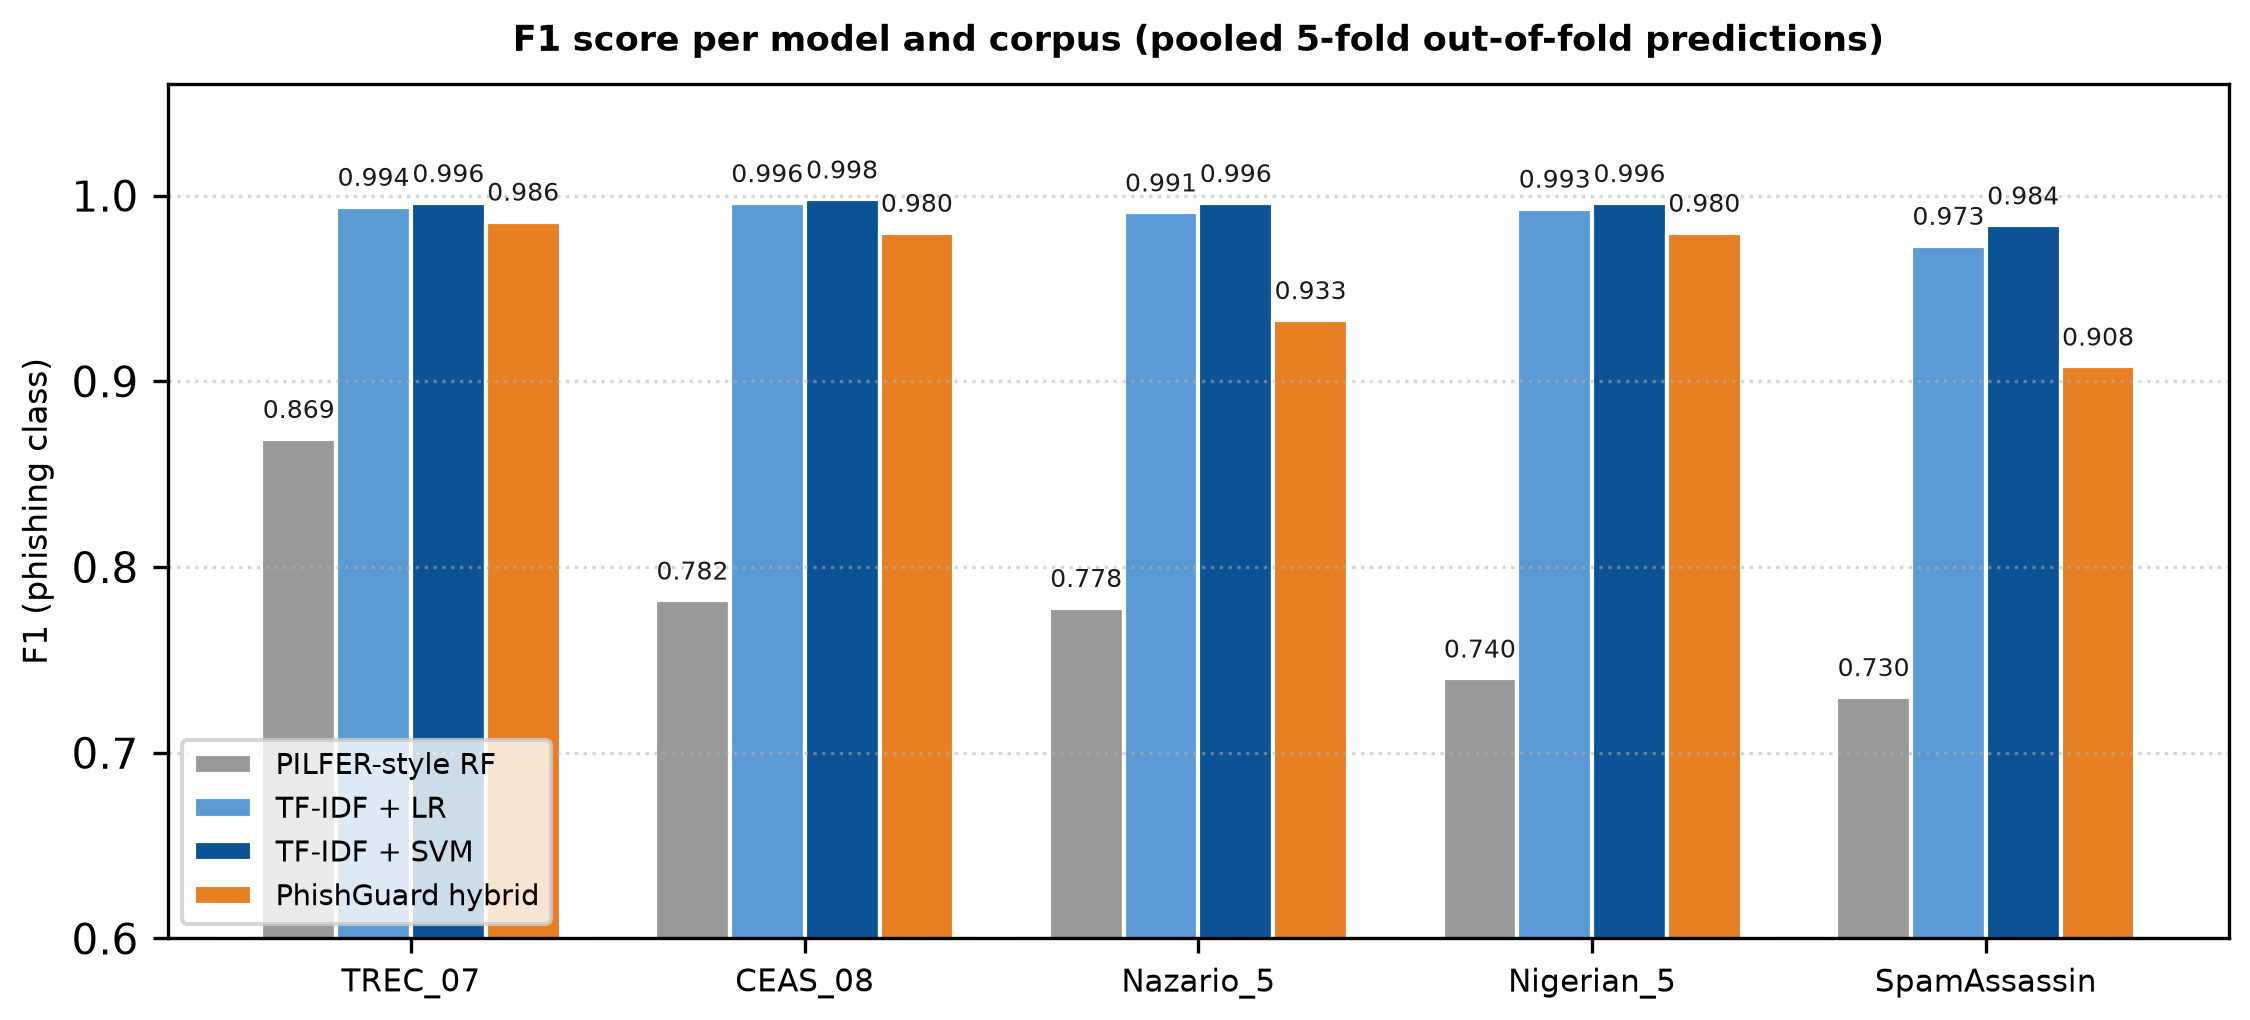
\includegraphics[width=\columnwidth]{fig_results.png}
\caption{F1 score per model and corpus (pooled 5-fold out-of-fold predictions).}
\label{fig:results}
\end{figure}

The two large corpora tell a consistent story. On TREC\_07 and CEAS\_08 every
model is strong. The hybrid takes the best precision observed anywhere, 0.996
and 0.999, with F1 of 0.986 and 0.980. Just behind the TF-IDF SVM on both.
Nazario\_5 shows the cost. Hybrid recall drops to 0.877 while precision holds
at 0.998. The rule layer's conservatism vetoes true positives its statistical
half would have caught. SpamAssassin is the hardest case for the hybrid:
recall 0.842, F1 0.908. That makes sense. It is general spam, not pure
phishing, and the rule engine is tuned for phishing indicators, so its
contribution shrinks. The PILFER-style baseline behaves the way classical
heuristics do. High recall, 0.836 to 0.964, with clearly lower precision,
0.624 to 0.949.

No claim of accuracy superiority here. The hybrid does not win on F1. What
the numbers show is a documented trade. The deterministic rule layer buys the
highest precision and per-indicator explanations at a recall cost of 1 to 14
points depending on the corpus. For triage work where false positives are
expensive analyst time, that is a defensible place to stand.

\section{Discussion, Limitations, and Future Work}
The corpora are binary. So the system's three-way output,
safe/suspicious/phishing, could not be fully evaluated. How the
\textit{suspicious} band behaves in practice is unmeasured. A graded-alert
corpus would be a worthwhile follow-up. The DistilBERT layer sat out this
build, untrained. Running it through the same protocol is the obvious next
experiment. The rule-engine thresholds and the 0.35/0.65 ensemble weights are
shipped defaults, never tuned. Per-deployment calibration should recover some
of the recall gap. Triage-time reduction in a real SOC is unmeasured. A
protocol for the author's SOC lab exists: 30 real Wazuh alerts, baseline
versus assisted triage, timed, with a washout period. The study has not run,
so no such claim is made. Finally, the corpora are English and partly dated.
Modern spear-phishing, non-English lures, and adversarial evasion of regex
rules are all untested.

\section{Conclusion}
PhishGuard is an open, deployable phishing triage platform. Its hybrid core,
evaluated on 108,116 public emails against three baselines, leads on
precision at 0.985 to 1.000 while trailing pure TF-IDF models on F1. An
honest, measured trade-off. It fits precision-sensitive SOC triage and
arrives with explanations an analyst can act on. Code, protocol, and results
are released for reproduction.

\section*{Acknowledgment}
The manuscript prose was drafted with the assistance of a generative AI
system (Muse, Meta) working from the author's system design, source code, and
measured benchmark results; the figures were produced with AI-assisted
scripting. All experimental results, numbers, and technical claims derive
from the author's own work. AI assistance was limited to drafting and
language; the research contribution is the author's own.

\begin{thebibliography}{00}
\bibitem{pilfer} I.~Fette, N.~Sadeh, and A.~Tomasic, ``Learning to detect
phishing emails,'' in \textit{Proc.\ 16th Int.\ Conf.\ World Wide Web (WWW)},
Banff, AB, Canada, 2007, pp.\ 649--656.
doi:\ 10.1145/1242572.1242660.

\bibitem{cantina} Y.~Zhang, J.~Hong, and L.~Cranor, ``Cantina: a content-based
approach to detecting phishing web sites,'' in \textit{Proc.\ 16th Int.\ Conf.\
World Wide Web (WWW)}, Banff, AB, Canada, 2007.

\bibitem{sahingoz2019} O.~K.~Sahingoz, E.~Buber, O.~Demir, and B.~Diri,
``Machine learning based phishing detection from URLs,''
\textit{Expert Syst.\ Appl.}, vol.\ 117, pp.\ 345--357, Mar.\ 2019.
doi:\ 10.1016/j.eswa.2018.09.029.

\bibitem{explicate} B.~Lim, R.~Huerta, A.~Sotelo, A.~Quintela, and P.~Kumar,
``EXPLICATE: Enhancing phishing detection through explainable AI and
LLM-powered interpretability,'' \textit{arXiv preprint arXiv:2503.20796
[cs.CR]}, 2025.

\bibitem{trec07} G.~V.~Cormack, ``TREC 2007 Spam Track overview,'' in
\textit{Proc.\ 16th Text REtrieval Conf.\ (TREC)}, NIST, Gaithersburg, MD,
2007.

\bibitem{phishcurated} \textit{Phishing Email Curated Datasets}, Zenodo,
doi:\ 10.5281/zenodo.8339691, 2023. {CC-BY-4.0}.
\end{thebibliography}

\end{document}
